\section{Sensor Nodes}

\begin{figure}[ht!]
   \centering
   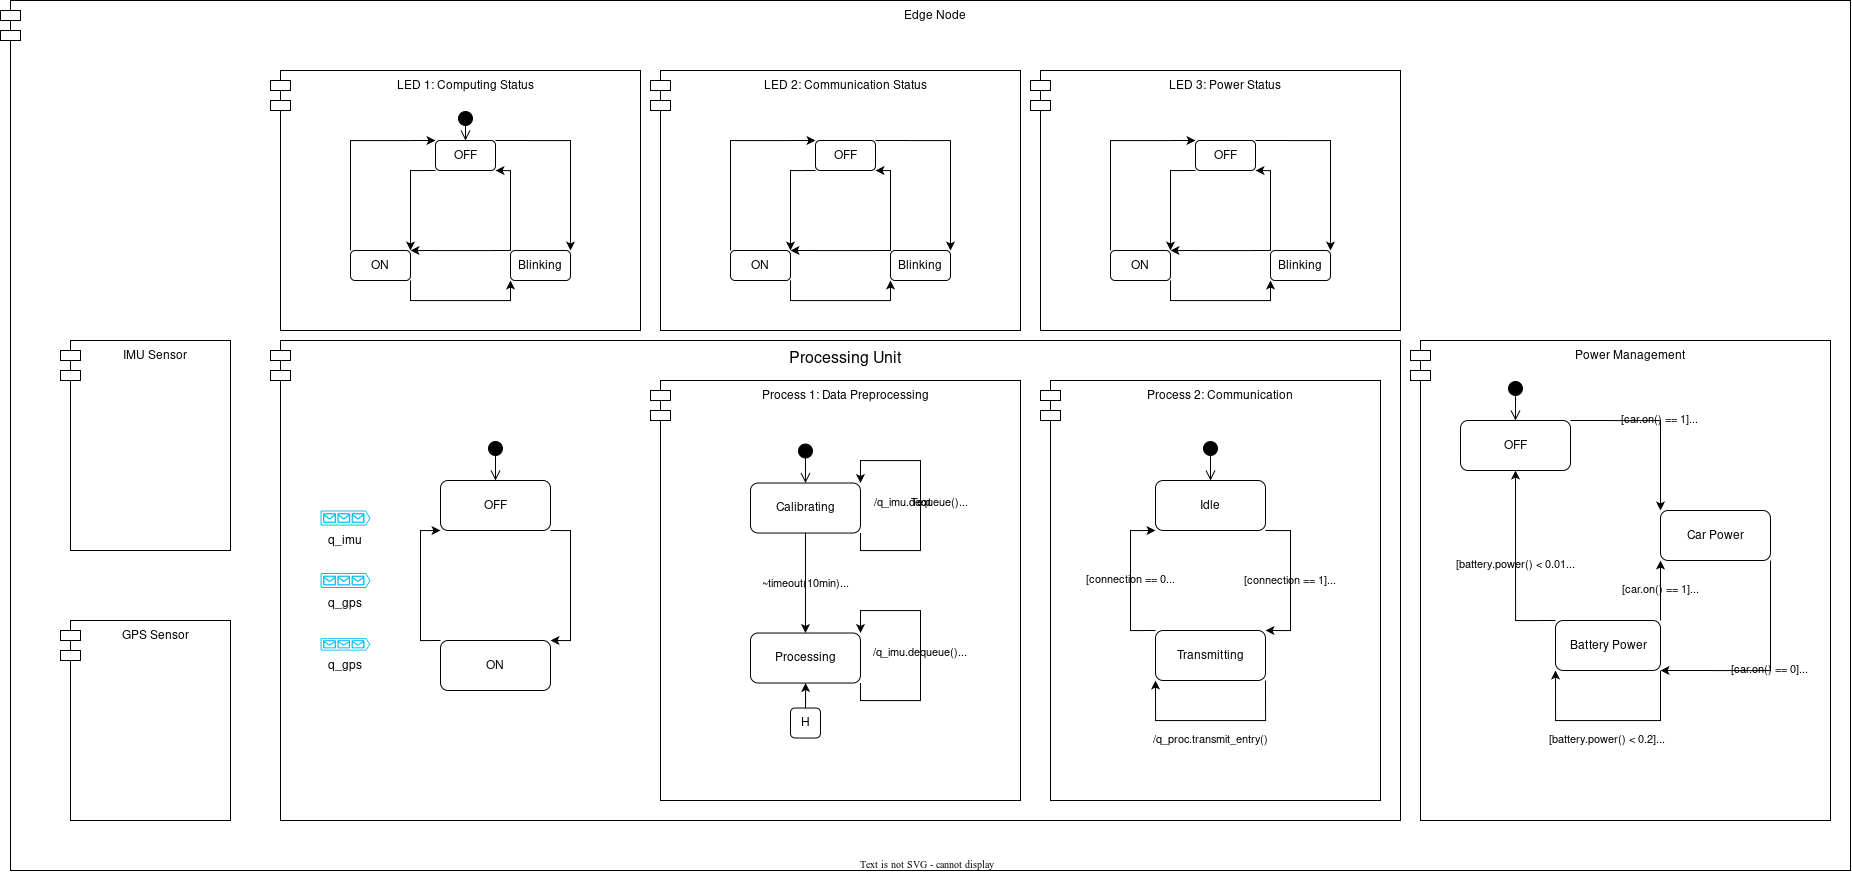
\includegraphics[width=\textwidth]{../../assets/diagrams/edge_node_rtuml/edge_node_rtuml.png}
   \hfill
   \caption{RT-UML of a Sensor Node}
   \label{fig:rt_uml_sensor_node}
\end{figure}

\subsubsection{Main Design Aspects}

\begin{enumerate}
    \item \textbf{Cost Restriction per node}: ~100 CHF  \\
      Given the large number of vehicles that will host sensor nodes, the cost per node must remain as low as possible. To achieve this, each vehicle will have a single sensor node/package installed to minimize installation and part costs.
      The qualification model is designed to be computationally efficient to minimize the cost of the microcontroller. Wifi connectability is chosen to minimize the cost of the communication module.

    \item \textbf{Quantification of Road State}: \\
      The sensor node will be ideally positioned centrally in the vehicle, above one of the axles, and securely mounted to the chassis to reduce measurement errors. The road state will be quantified on a scale from 0 (very good) to 244 (very poor), with 255 reserved for hazardous conditions.
    
   \item \textbf{Qualification Model}: \\
      \begin{align}
         \text{RoadQuality}_i =  \lfloor \frac{max(\Delta a_{z,t}) - \Delta a_{z,\text{min}}}{\Delta a_{z,\text{max}} - \Delta a_{z,\text{min}}} \rfloor  \cdot 255 \quad \text{where} \quad  t \in \text{RoadSegment}_i
      \end{align}

      This model is based on the assumption that the maximum acceleration in z-axis is proportional to the road quality.
      By calculating the acceleration difference between the current and the previous time step, the model is unaffected by the vehicle's orientation and acceleration.
      $\Delta a_{z,\text{min}}$ and $\Delta a_{z,\text{max}}$ are determined during the calibration phase and symbolize the minimum and maximum acceleration difference occurring during possible driving conditions. 
      This makes the model adaptable to different vehicles and driving conditions. \\

      Future iterations will adapt a simulation based approach described in the following: \\
      A simple linear Mass-Spring-Damper Model is chosen to model the cars factor on the transduced shocks. (While keeping computational effort low.)
      A first calibration phase coupled to a initial parameter set aims to fit Mass-Spring-Damper Model parameters.
      Measured data will be fit to quantified values during calibration phase.
      Further physical quatities other than z-axis acceleration have to be considered to decouple driving induced accelerations from the road state.
    
   \item \textbf{High Polling Rate for IMU Measurements}: \\
      Road-induced shocks are brief and their period and amplitude are proportional to vehicle speed. The IMU's polling rate will be configured to ensure reliable readings for typical driving speeds.
      Currently the acceleration is measured every 3ms, acchieving a road resolution of 2.5cm at 30 km/h which is the assumed avrage speed in urban areas.
    
   \item \textbf{Sensing of physical quantities}:
      The system will measure multiple physical quantities to ensure accurate road state assessments:
      \begin{enumerate}
      \item \textbf{Acceleration in z-Axis} to determine road state and potholes.
      \item \textbf{Acceleration in x,y-Axis and rotational acceleration} to minimize errors induced from driving scenarios. (Possible part of future work)
      \item \textbf{Driving Velocity} to approximate relative distance through integration needed for velocity indipendent Segmentation of QualityMeasures. \\ (Future Work: to couple shock amplitudes to velocity through Spring-Damper Model).
      \item \textbf{Geographical Position} to reference qualification to current position.
      \end{enumerate}
    
   \item \textbf{Data Transmission at Established Gatepoints}: \\
      \begin{enumerate}
          \item \textbf{Data Format}: Each data package will include the following information encoded as a JSON object:
            \begin{lstlisting}[breaklines=true, basicstyle=\ttfamily]
(Node ID (2 Bytes)) |
 Position (2 x 8 Bytes (Double-Precision Float)) | Road Quality (1 Byte) | Unix Timestamp (4 Bytes)
            \end{lstlisting}

            For example, the following snippet represents a valid data sample in JSON format:

            \begin{lstlisting}[breaklines=true, basicstyle=\ttfamily]
               {               
               "lat": 46.19313,
               "lon": 6.80421,
               "timestamp": 1734478933,
               "bumpiness": 50,
               "device_id": "USI-Car-1""
               }
            \end{lstlisting}

          \item \textbf{Local Preprocessing}: The node will preprocess and store position-quality tuples locally.
          \item \textbf{Gatepoint Connectivity}: The node will automatically establish a connection at predefined gatepoints to transmit new data.
          \item \textbf{Data Protocol}: Data packages will be transmitted in MQTT format to a RabbitMQ server.
      \end{enumerate}
    \end{enumerate}